\documentclass[tikz,border=5mm]{standalone}
\usepackage{tikz}
\usetikzlibrary{calc,patterns}

\begin{document}
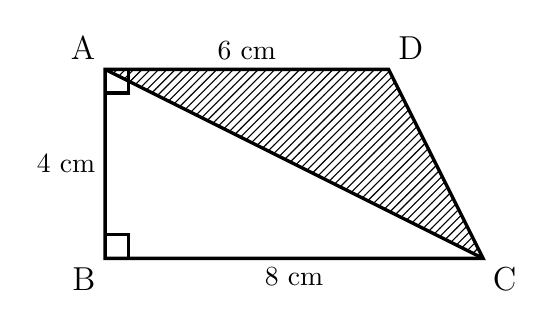
\begin{tikzpicture}[scale=1.2]

% Define vertices
\coordinate (A) at (0,2);
\coordinate (B) at (0,0);
\coordinate (C) at (4,0);
\coordinate (D) at (3,2);

% Fill triangle ACD with diagonal hatching
\fill[pattern=north east lines] (A) -- (C) -- (D) -- cycle;

% Draw trapezoid ABCD
\draw[very thick] (A) -- (B) -- (C) -- (D) -- cycle;

% Draw diagonal AC
\draw[very thick] (A) -- (C);

% Right angle mark at B (inside)
\draw[very thick] (B) ++(0.25,0) -- ++(0,0.25) -- ++(-0.25,0);

% Right angle mark at A (inside)
\draw[very thick] (A) ++(0.25,0) -- ++(0,-0.25) -- ++(-0.25,0);

% Vertex labels
\node[above left] at (A) {\large A};
\node[below left] at (B) {\large B};
\node[below right] at (C) {\large C};
\node[above right] at (D) {\large D};

% Side labels (in English)
\node[above] at ($(A)!0.5!(D)$) {6 cm};
\node[left] at ($(A)!0.5!(B)$) {4 cm};
\node[below] at ($(B)!0.5!(C)$) {8 cm};

\end{tikzpicture}
\end{document}